\documentclass[12pt]{article}

\usepackage[italian]{babel} 
\usepackage[utf8x]{inputenc}
\usepackage{graphicx}
\usepackage{cleveref}
\usepackage{wrapfig}
\usepackage{hyperref}
\usepackage{multicol}

\graphicspath{ {images/} }

\pagestyle{headings}
\title{R2Pi0}
\author{
  Tosatto Davide
  \and
  Riccardo Grespan
}


\newcommand{\cbegin}{‘‘}
\newcommand{\cend}{’’}
\newcommand{\imgsz}{0.3\textwidth}
\newcommand{\imgszland}{0.6\textwidth}
\newcommand{\raspi}{Raspberry Pi} 
\newcommand{\raszero} {\raspi{} Zero}

\makeindex

\begin{document} 


\maketitle
\newpage
\tableofcontents
\newpage
\section{Obiettivi del progetto}

\begin{minipage}{\linewidth}
L'intera documentazione in formato \LaTeX è disponibile nella repo \url{https://github.com/Tosa95/R2Pi0_Doc.git}.
\end{minipage}

\bigskip

L'obiettivo del progetto è di creare una riproduzione in scala di R2-D2, noto personaggio robotico della serie di Star Wars.

\begin{figure}[h]
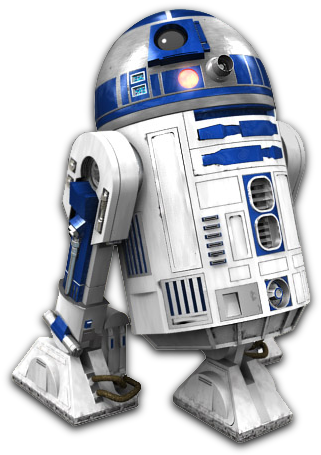
\includegraphics[width=\imgsz]{R2D2}
\centering
\caption{R2D2}
\label{fig:R2D2}
\end{figure}

La ricostruzione comprende:
\begin{enumerate}
\item movimento sul piano attraverso ruote;
\item riproduzione di suoni simili a quelli originali attraverso un buzzer, per dare quel tocco di retro che non guasta mai;
\item luci led e finto proiettore, comunque emulato da un led;
\item rilevamento degli ostacoli e corrispondente arrabbiatura del robot se viene mandato a tutta velocità verso uno di essi;
\item funzione follow che permette di mantenere una certa distanza dall'oggetto (o dalla persona) che lo precede
\item controllo vocale per funzioni base;
\item esoscheletro in cartone e plastica che riproduce le fattezze del robot;
\item un abbozzo di emozioni per dare un minimo di personalità al robot.
\end{enumerate}

Questa prima versione non avrà la possibilità di ruotare la testa e cambiare inclinazione, questo per mancanza di tempo e di componenti (ulteriori motori, ulteriori driver, contatti girevoli per le luci posizionate sulla testa)
 
\section{Componenti e scelte progettuali}
\subsection{Scheda di controllo}
Iniziamo dal cuore del progetto: \emph{la scheda di controllo}.

Le opzioni erano sostanzialmente due: \raszero{} o Arduino Uno.

\begin{figure}[h]
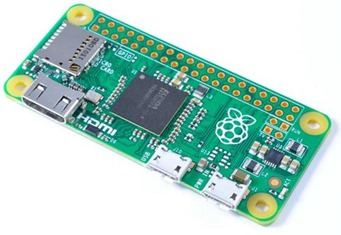
\includegraphics[width=\imgsz]{rpi0}
\centering
\caption{\raszero}
\label{fig:rpi0}
\end{figure}

\begin{figure}[h]
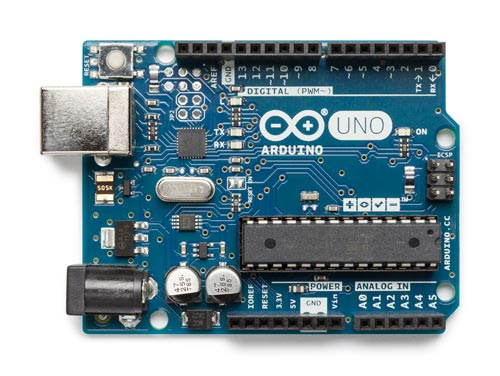
\includegraphics[width=\imgsz]{Uno}
\centering
\caption{Arduino Uno}
\label{fig:uno}
\end{figure}

Per la maggior parte dei compiti le due schede erano sostanzialmente intercambiabili, in particolare:
\begin{enumerate}
\item \emph{GPIO - General Purpose Input Output}: entrambi i dispositivi hanno tutte le interfacce che ci servono, ossia qualche I/O digitale e uscite PWM. Entrambi non possono dare in uscita elevate correnti, ma questo non importa perché il controllo di ogni componente è sempre mediato da transistor esterni;
\item \emph{Alimentazione}: entrambi i dispositivi possono essere alimentati da usb, rendendo quindi possibile l'utilizzo di una batteria esterna per cellulare;
\item \emph{Potenza di calcolo}: entrambi i dispositivi in esame hanno la potenza di calcolo necessaria per svolgere ognuno dei compiti necessari agli scopi del progetto.
\end{enumerate} 

Le seguenti motivazioni ci hanno fatto propendere per \raszero :
\begin{enumerate}
\item \emph{Semplicità di sviluppo}: grazie al fatto di avere a disposizione un sistema operativo completo, possiamo utilizzare linguaggi di più alto livello rispetto al C fornito da Arduino. Questo ci permette di creare codice meglio organizzato e più facilmente espandibile in futuro. La nostra scelta per il linguaggio è ricaduta su \emph{Python}, in quanto semplice, conciso ed efficace;
\item \emph{Memoria a disposizione}: grazie alla memoria disponibile, sensibilmente superiore a quella di Arduino, ci è permesso di integrare più suoni. Inoltre, in futuro, sarà sempre possibile migliorare la qualità degli stessi.
\item \emph{Facilità di connessione}: \raszero{} risulta più facile da connettere al mondo in quanto basta collegare un adattatore USB per WiFi o Bluetooth. Arduino invece richiede specifici shield,.
\item \emph{Prezzo}: \raszero{} costa 5\$, molto meno di un Arduino, e offre infinite possibilità grazie ad un sistema operativo completo.
\end{enumerate}

Un notevole problema del \raszero{} e' il consumo.

Arduino senza carico consuma circa 50mA, mentre \raszero{} arriva a 65mA in idle, si alza parecchio se il carico di lavoro aumenta, in quanto il processore di \raszero{} è molto più performante di quello di Arduino, inoltre, montando un sistema operativo completo, \raszero{} ha anche diverso overhead in campo di potenza computazionale e consumo, cosa non trascurabile.

Chiaramente i dispositivi di comunicazione comportano un innalzamento dei consumi in entrambe le schede.

Per ridurre al minimo i consumi abbiamo installato Raspbian in versione lite, ossia senza interfaccia grafica, e disattivato il controllore video HDMI, guadagnando così qualche prezioso mA.

In conclusione, i vantaggi nell'utilizzo di \raszero{} ci sono sembrati schiaccianti.

\subsection{Comunicazione}
Le due opzioni per la comunicazione sono: Bluetooth o WiFi.

Abbiamo optato per una connessione Bluetooth per i seguenti motivi:
\begin{enumerate}
\item \emph{Consumo}: il Bluetooth risulta avere un consumo energetico inferiore rispetto al WiFi, portandoci ad avere una durata della batteria leggermente superiore (non abbiamo dati precisi).
\item \emph{Semplicità d'uso}: il Bluetooth è pensato per connessioni punto a punto, ossia esattamente la funzione che serve a noi. Il Wifi, invece, non è pensato per quello scopo e quindi relegherebbe all'utilizzo nei soli spazi dotati di rete WiFi oppure alla configurazione di una rete ad-hoc che risulta comunque un'operazione non banale e spesso mal funzionante (soprattutto su Linux).
\end{enumerate}

\bigskip
\bigskip

NOTA: sebbene fosse sicuramente preferibile utilizzare un adattatore BLE, meno energivoro, per ragioni di componentistica disponibile abbiamo dovuto optare per un vecchio adattatore Bluetooth 2.0.\\
Inoltre, data la recente uscita del \raszero{} W, con lo stesso hardware di Pi Zero, ma dotato anche di BLE e WiFi, al costo (teorico) di 10\$, avremmo potuto usare tale dispositivo, ma per mancanza di disponibilità e costi di spedizione superiori al suo valore, abbiamo deciso di rimanere sul Pi Zero di prima generazione. 

\section{Schemi circuitali}

Benchè \raspi{} sia spesso usato come microcontrollore, in realtà non è propriamente tale, si avvicina molto più ad un PC standard che ad una MCU.

Non è quindi in grado di erogare grandi correnti sui suoi pin di I/O. Non esiste un vero e proprio datasheet che dia dei valori precisi, ma nella community di sviluppatori \raspi{} si danno per accettate le seguenti soglie:
\begin{itemize}
\item circa 10-15mA per piedino
\item circa 50mA di assorbimento complessivo derivante dalla somma dei contibuti di tutti i piedini
\item i piedini a 5V sono collegati direttamente all'alimentazione, quindi da essi si può assorbire tutta la corrente erogabile dall'alimentatore meno quella assorbita dal \raspi{} stesso
\end{itemize}

Da questi valori si può capire come le uscite del \raspi{} siano state ideate per essere bufferate, e così noi abbiamo fatto.

\subsection{Controllo motori}
Per il controllo dei motori abbiamo deciso di utilizzare una versione leggermente modificata del ponte H. I nomi dei componenti sono presi da \cref{fig:ponteH}. \'E necessario uno di questi circuiti per ogni motore installato.

\begin{figure}[h]
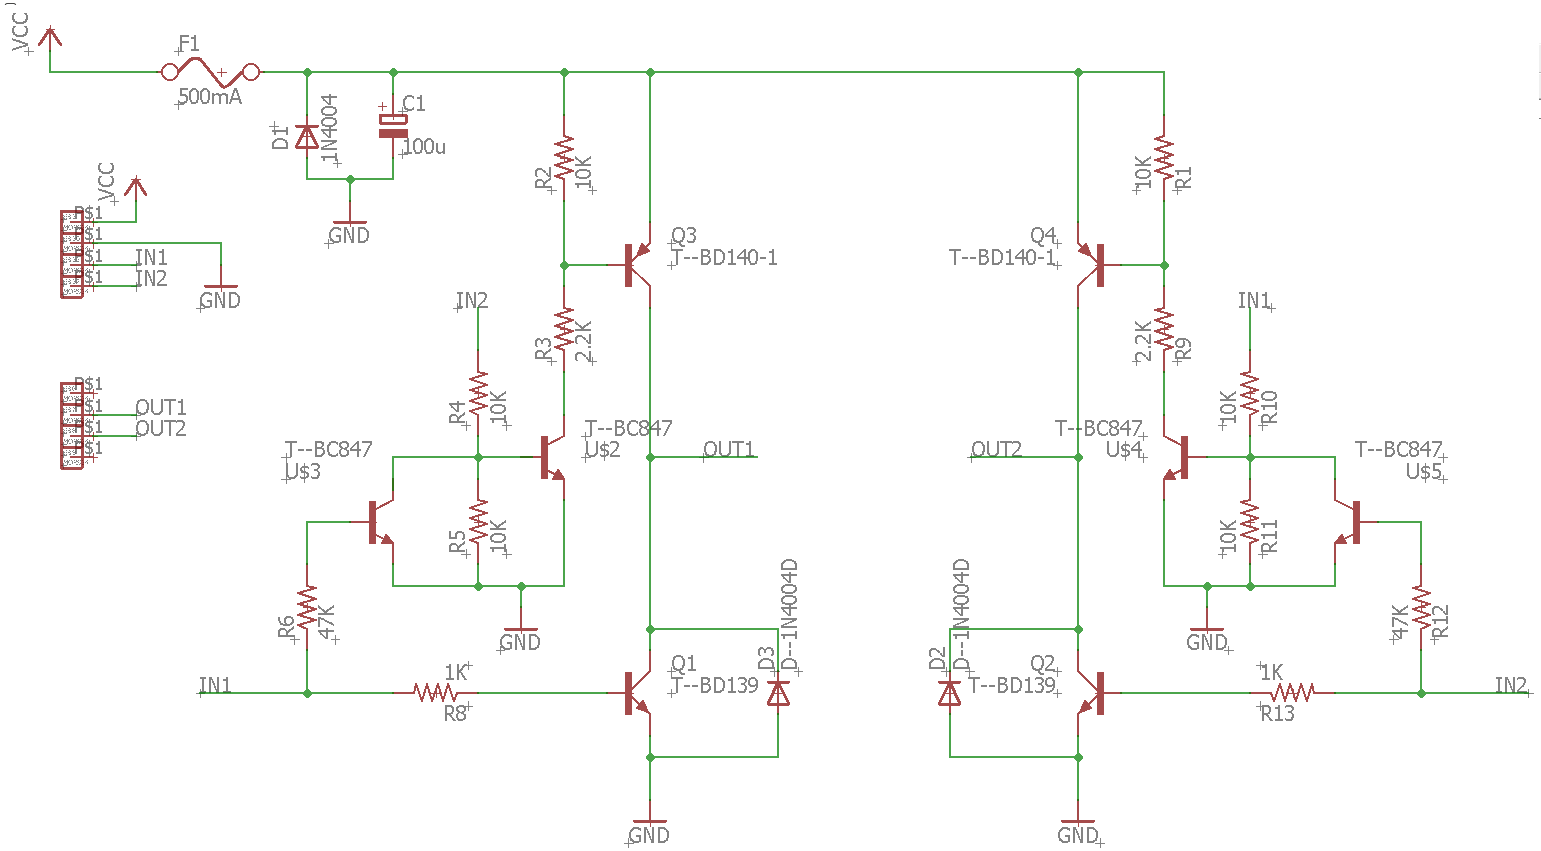
\includegraphics[width=\textwidth]{SchemaH}
\centering
\caption{Schema del circuito di controllo dei motori}
\label{fig:ponteH}
\end{figure}

Passiamo alla rapida spiegazione del funzionamento del circuito. Il circuito ha due input: IN1 e IN2. Il comportamento è il seguente:
\begin{enumerate}
\item Se solo uno dei due fra IN1 e IN2 è attivo, nel motore scorre corrente, il verso dipende da quale dei due è alto.
\item Se sia IN1 che IN2 sono a 0, il motore resta completamente scollegato dal circuito, permettendogli di muoversi per inerzia.
\item Se sia IN1 che IN2 sono a 1, il motore ha entrambi i terminali a massa. Questo chiude la bobina del motore creando un cortocircuito. Così facendo se si tenta di muovere il motore si originerà all'interno della bobina una corrente che genererà a sua volta un campo magnetico che si opporrà al movimento del motore. Questo ha come risultato un effetto frenante. 
\end{enumerate}

Passiamo alla disamina dei componenti e delle loro funzioni.
Tutti i transistori sono BJT, perché permettono di fare passare correnti elevate e soprattutto hanno basse cadute di potenziale in saturazione, ossia circa 0.3V tra collettore ed emettitore. Mantenere cadute di potenziale basse è essenziale perché il tutto è alimentato a soli 5V.

I quattro transistor principali di potenza sono Q1, Q2, Q3 e Q4. La circuiteria è fatta in modo tale che né Q1 e Q3, né Q2 e Q4 conducano \emph{mai} insieme. Questo avvenimento infatti produrrebbe un cortocircuito che danneggerebbe l'hardware.

Da misurazioni, si è visto che il consumo di ogni motore è inferiore ai 200mA, si è dunque pensato di inserire per sicurezza un fusibile da 500mA, F1, sufficientemente permissivo da far funzionare il motore, ma abbastanza restrittivo per evitare di bruciare l'alimentatore in caso di corto.

Abbiamo poi altri quattro transistor che servono ad assicurare l'assenza di corti e ad implementare la funzionalità di cortocircuitare la bobina con entrambi gli ingressi a 1.\\
La funzione logica realizzata è quella mostrata in tabella \ref{tab:tabFunz}

\begin{table}[h]
\begin{center}


\begin{tabular}{l|l|l|l|l|l}

IN1 & IN2 & Q1 & Q2 & Q3 & Q4 \\
\hline
off & off & off & off & off & off \\
off & on & off & on & on &  off \\
on & off & on & off & off &  on \\
on & on & on & on & off & off


\end{tabular}

\end{center}
\caption{Funzione logica implementata nel circuito}
\label{tab:tabFunz}
\end{table}

Da notare che U\$2 e U\$4 hanno un partitore resistivo sulla base. Questo serve a ritardare la loro accensione, infatti gli input non sono realmente squadrati ma aumentano gradualmente con una certa pendenza, seppur elevata. Questo permette di ritardare l'attivazione dei transistor sopracitati. Infatti se sulla base servono 0.7V per permettere l'accensione, con il partitore è richiesto che IN2 sia già ad almeno 1.4V. Questo accorgimento serve quando attiviamo contemporaneamente IN1 e IN2, per dare il tempo a U\$3 e U\$1 di inibire l'accensione di Q3 e Q4 impedendo quindi cortocircuiti.

\subsection{Buzzer}

Abbiamo usato un buzzer piezoelettrico recuperato da un vecchio telefono.

Dal datasheet del buzzer emerge la seguente figura:
\begin{figure}[h]
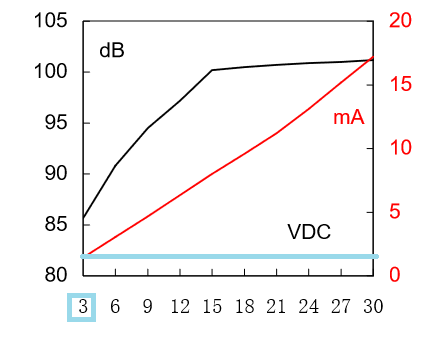
\includegraphics[width=\imgszland]{buzzerDS}
\centering
\caption{Caratteristica tensione-corrente del buzzer}
\label{fig:buzzerDS}
\end{figure}

Considerando che lavoriamo attorno ai 3V, dal grafico possiamo notare come, a tale tensione, la corrente assorbita sia di circa 2mA.\\
Possiamo quindi lasciare che il buzzer sia pilotato direttamente dal \raspi{} in quanto, come detto ad inizio sezione, ogni piedino può erogare fino a 10mA, quindi siamo ampiamente entro la soglia.

\subsection{Sensore di prossimità}

\begin{figure}[h]
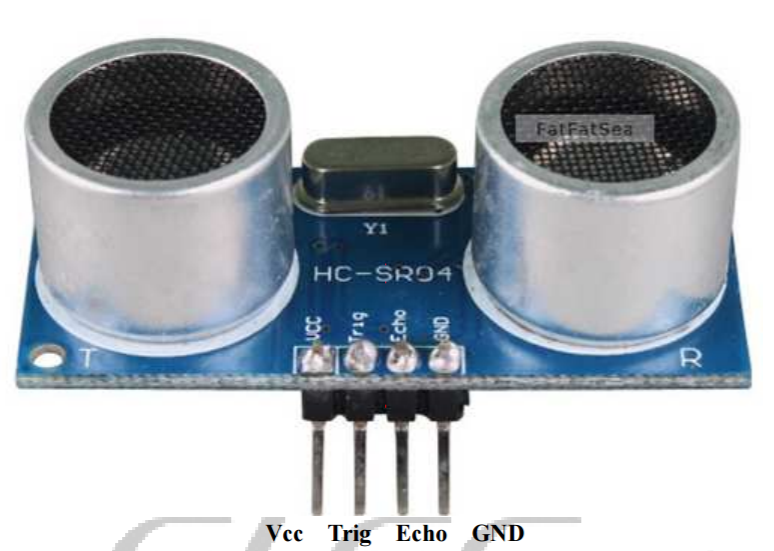
\includegraphics[width=\imgszland]{us_img}
\centering
\caption{Sensore di prossimità}
\label{fig:buzzerDS}
\end{figure}

Il rilevatore di distanza del robot è un sensore ad ultrasuoni HC-SR04.
\'E costituito da un emettitore e da un ricevitore di ultrasuoni, gestiti da un circuito di controllo.\\
Emette ultrasuoni ad una frequenza di 40KHz. Può misurare distanze dai 2cm fino ai 4m, con un angolo di 15 gradi e una precisione fino a 3mm, perfetto per le misurazioni che dobbiamo effettuare.\\
Per la connessione e l'utilizzo è dotato di 4 pin:
\begin{itemize}
\item VCC: alimentazione a 5V;
\item GND: massa;
\item Trig: input per scatenare l'inizio della rilevazione;
\item Echo: output per l'invio della distanza alla board, codificato come impulso di durata variabile.
\end{itemize}

\begin{figure}[h]
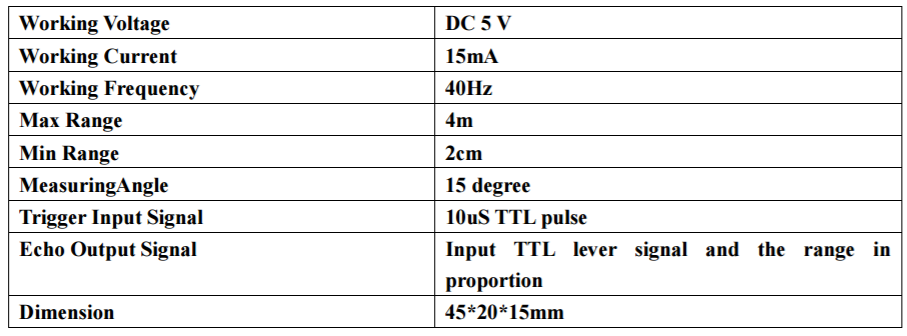
\includegraphics[width=\linewidth]{us_data}
\centering
\caption{Caratteristiche di interfacciamento del sensore di prossimità}
\label{fig:usdata}
\end{figure}



Come possiamo notare in \autoref{fig:usdata}, il sensore usa i livelli tipici della logica TTL.

Infatti, funziona ad un voltaggio di 5V. Questo non è un problema in quanto su \raspi{} abbiamo una linea di alimentazione a 5V liberamente usabile.

I problemi sorgono nell'interfacciamento dati tra \raspi{} e sensore.\\
Per quanto riguarda il piedino Trig, di input per il sensore, non ci sono problemi in quanto la Vih dei TTL si attesta intorno ai 2V, quindi con i 3.3V (circa) di output di \raspi{} riusciamo a pilotarlo senza problemi.\\
Il piedino Echo mostra invece qualche problema in più, in quanto i piedini di input del \raspi{} non sono 5V-tolerant. Se collegato direttamente potrebbe quindi danneggiare la board. Per evitare questo problema abbiamo utilizzato un semplice partitore resistivo con $R2 = 2R1$, in modo da moltiplicare la tensione per un fattore $2/3$: $5V*(2/3)=3.3V$, come desiderato.

\begin{figure}[h]
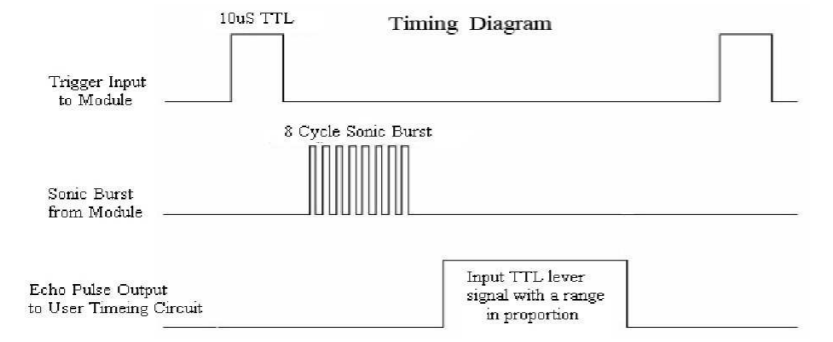
\includegraphics[width=\linewidth]{us_diagram}
\centering
\caption{Diagramma temporale del sensore di prossimità}
\label{fig:usdiagram}
\end{figure}

Per effettuare la misurazione è necessario inviare un segnale dal Raspberry Pi al pin trigger del sensore della durata minima di 10us, il segnale verrà poi emesso come ultrasuono che rimbalzando contro una superficie verrà riflesso e captato dal ricevitore. 
Il sensore risponderà poi al \raspi{} sul pin Echo con un impulso di durata proporzionale alla distanza dell'ostacolo dal sensore.

Per il calcolo si usa la seguente formula:\\
\begin{center}
$ distanza = durataEcho * SOUND\_CONST $
\end{center}
dove:
\begin{itemize}
\item $SOUND\_CONST$ è un valore costante di conversione (171.5)
\item $durataEcho$ è la durata dell'impulso misurato sul piedino Echo, in seocndi
\item $distanza$ è la distanza, in metri dall'ostacolo
\end{itemize}





\section{Software}

\subsection{Lato \raspi}

\begin{minipage}{\linewidth}
Tutto il codice sorgente lato \raspi{} è liberamente accessibile attraverso il seguente repository github:  \url{https://github.com/vxrich/Python_R2Pi0.git}.
\end{minipage}

Il codice è commentato, ma solo nei punti in cui abbiamo ritenuto necessario precisare qualcosa. Per le funzioni o le classi autoesplicative abbiamo evitato di aggiungere commenti, in modo da non appesantire la lettura del codice.

Si è deciso di dare al software un'impronta un po' più professionale rispetto al semplice script dimostrativo autocontenuto.\\
Abbiamo quindi suddiviso il codice in diversi moduli e usato alcuni design patterns per rendere il software il più possibile espandibile in futuro. Ovviamente resta un progetto di piccole dimensioni, senza particolari complessità.

Vediamo una rapida disamina dei moduli software:
\begin{enumerate}
\item \emph{Controllo del movimento}: questo è un macro modulo composto da diversi sottomoduli. Abbiamo deciso di realizzare il controllo dei motori attraverso un decorator pattern: abbiamo uno stack liberamente componibile di controllori che via via aggiungono funzionalità. La classe base \emph{MotionController} astrae il controllo vedendolo come una semplice combinazione di una velocità ed una rotazione. Aggiunge inoltre un \emph{watchdog} per essere certi che, in assenza di comandi per un certo periodo di tempo, il robot venga fermato. Abbiamo poi il layer \emph{DistanceAdapter} che aggiunge la funzionalità di blocco in caso di ostacoli e il layer \emph{MoodedAdapter} che aggiunge alcuni semplici comportamenti \cbegin{}emotivi\cend{} del robot.\\
\begin{figure}[h]
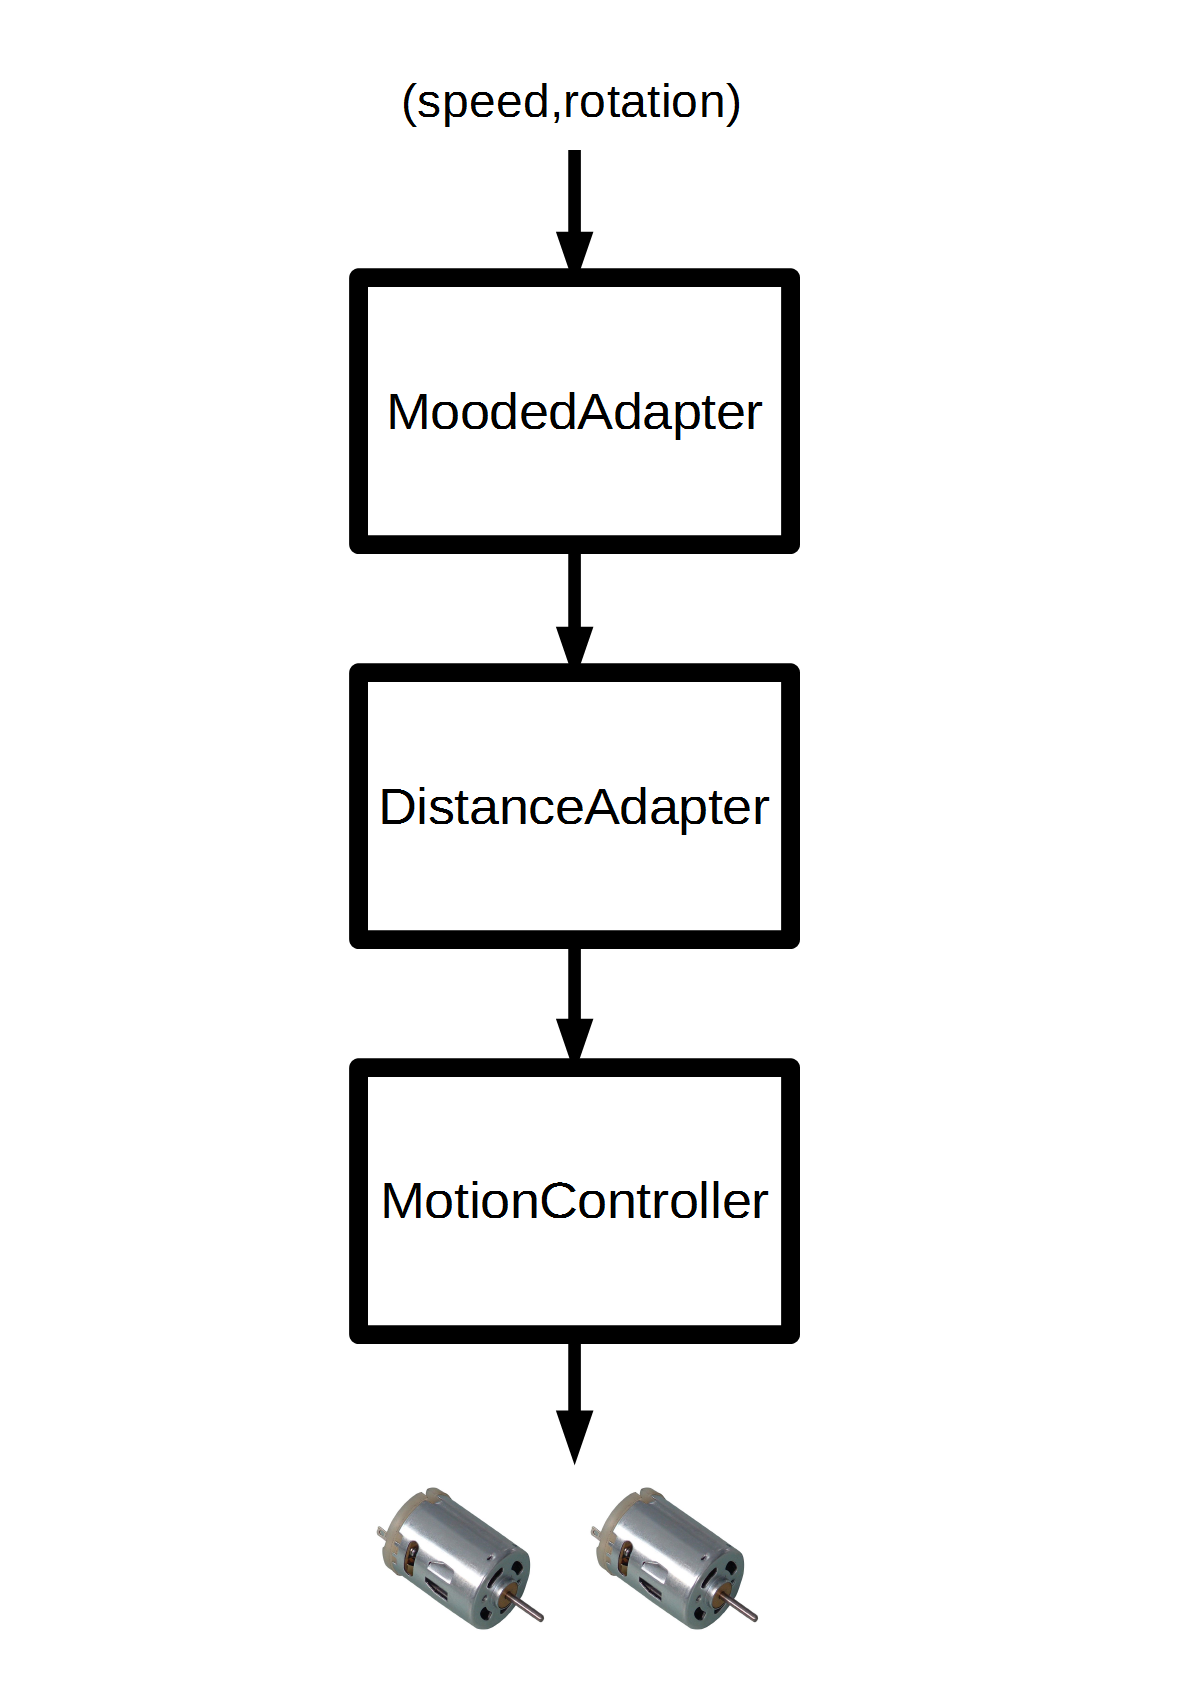
\includegraphics[width=\imgszland]{motion_stack}
\centering
\caption{Stack controllo movimento usato nella versione attuale}
\label{fig:motion_stack}
\end{figure}
Ci sono poi i sottomoduli \emph{Follower} e \emph{Reacher} che si occupano rispettivamente di mantenere una certa distanza dall'ostacolo di fronte e di raggiungerlo (attivati mediante comando vocale dall'app Android).
\item \emph{Server}: composto essenzialmente da due classi: \emph{Server} e \emph{Subserver}. Server rimane in ascolto sul bluetooth e per ogni nuova connessione avvia una nuova istanza di Subserver che si occuperà di soddisfare le richieste del client.\\
Ricevono in ingresso un array associativo contenente coppie comando-callback, in modo da poter aggiungere e togliere comandi nel modo più semplice possibile.
\item \emph{Suono}: Si occupa di gestire la riproduzione di suoni monofonici in formato RTTTL. Composto da due classi: \emph{RTTLConverter}, che converte i file RTTTL in un formato più usabile in runtime ed \emph{RTTLPlayer}, che prende in input i suoni convertiti e li esegue in sequenza (ha una coda di esecuzione).
\item \emph{Sensore di prossimità}: questo modulo è stato il più critico, perchè, per leggere la distanza, è necessario misurare la durata di un impulso su un pin di I/O. Scritto in python, questo risultava troppo CPU intensive, in quanto dovevamo di fatto eseguire un polling sul piedino senza poter mettere in pausa il thread per non avere enormi perdite di precisione.\\
La soluzione è stata di ricorrere alla libreria \emph{wiringPi}, che, nella sua declinazione per il linguaggio C, permette di utilizzare degli interrupt scatenati sui fronti di salita e/o discesa dei pin di I/O.\\
Abbiamo quindi scritto questo particolare modulo in C, poi un wrapper per poterlo compilare come modulo Python. Un po' una faticaccia ma il risultato è ottimo!\\
Il modulo C si chiama \emph{proxsensor}, mentre in Python lo abbiamo incapsulato nella classe \emph{SensorController} (del modulo UltrasonicSensor.py) che legge la distanza ad intervalli regolari, scatenando un evento con la nuova distanza a cui si possono collegare tutti i listener del caso (pattern Observer).
\item \emph{Mood}: piccolo modulo che ha il compito di gestire qualche emozione del robot. Niente di che, andrebbe ampliato.
\item \emph{Pinout}: questo modulo contiene \emph{tutte} le associazioni pin-funzione svolta necessarie per il progetto. Questo ci permette di rimappare tutti gli I/O velocemente attraverso un singolo file.
\item \emph{Blue}: alcune funzioni di utilità per utilizzare la connessione bluetooth.
\item \emph{Misc}: cartella contente note ed appunti su come preparare un \raspi{} per fare funzionare questa applicazione.
\item \emph{r2pi0\_{}V2}: punto di ingresso del sistema. \'E lo script da lanciare (con permessi di amministratore) per fare funzionare il tutto.

Quasi tutti i moduli sono connessi attraverso eventi e rispettivi callback per ridurre al minimo possibile l'interdipendenza tra gli stessi.
\end{enumerate}

\subsection{Lato Smartphone}

\begin{minipage}{\linewidth}
Tutto il codice sorgente lato Smartphone è liberamente accessibile attraverso il seguente repository github: \url{https://github.com/vxrich/R2-Pi0.git}.
\end{minipage}

Il codice è commentato, ma solo nei punti in cui abbiamo ritenuto necessario precisare qualcosa. Per le funzioni o le classi autoesplicative abbiamo evitato di aggiungere commenti, in modo da non appesantire la lettura del codice.

La nostra riproduzione di R2-D2 necessita di un controller remoto per i movimenti e le interazioni base,
per questo abbiamo deciso di utilizzare un'applicazione programmata ad hoc per smartphone.

L'applicazione e' scritta in \emph{Java} per sistema operativo \emph{Android}.

\medskip

Partendo dalla parte visiva, l'applicazione e' costituita da elementi grafici per l'interazione con il robot, che permettono:
\begin{itemize}
\item il controllo del movimento tramite un joystick virtuale
\item l'attivazione della connessione bluetooth con la macchina
\item l'invio di una richiesta per la riproduzione di suoni
\item l'attivazione dei comandi vocali
\item lo spegnimento completo del robot
\end{itemize}

\begin{figure}[h]
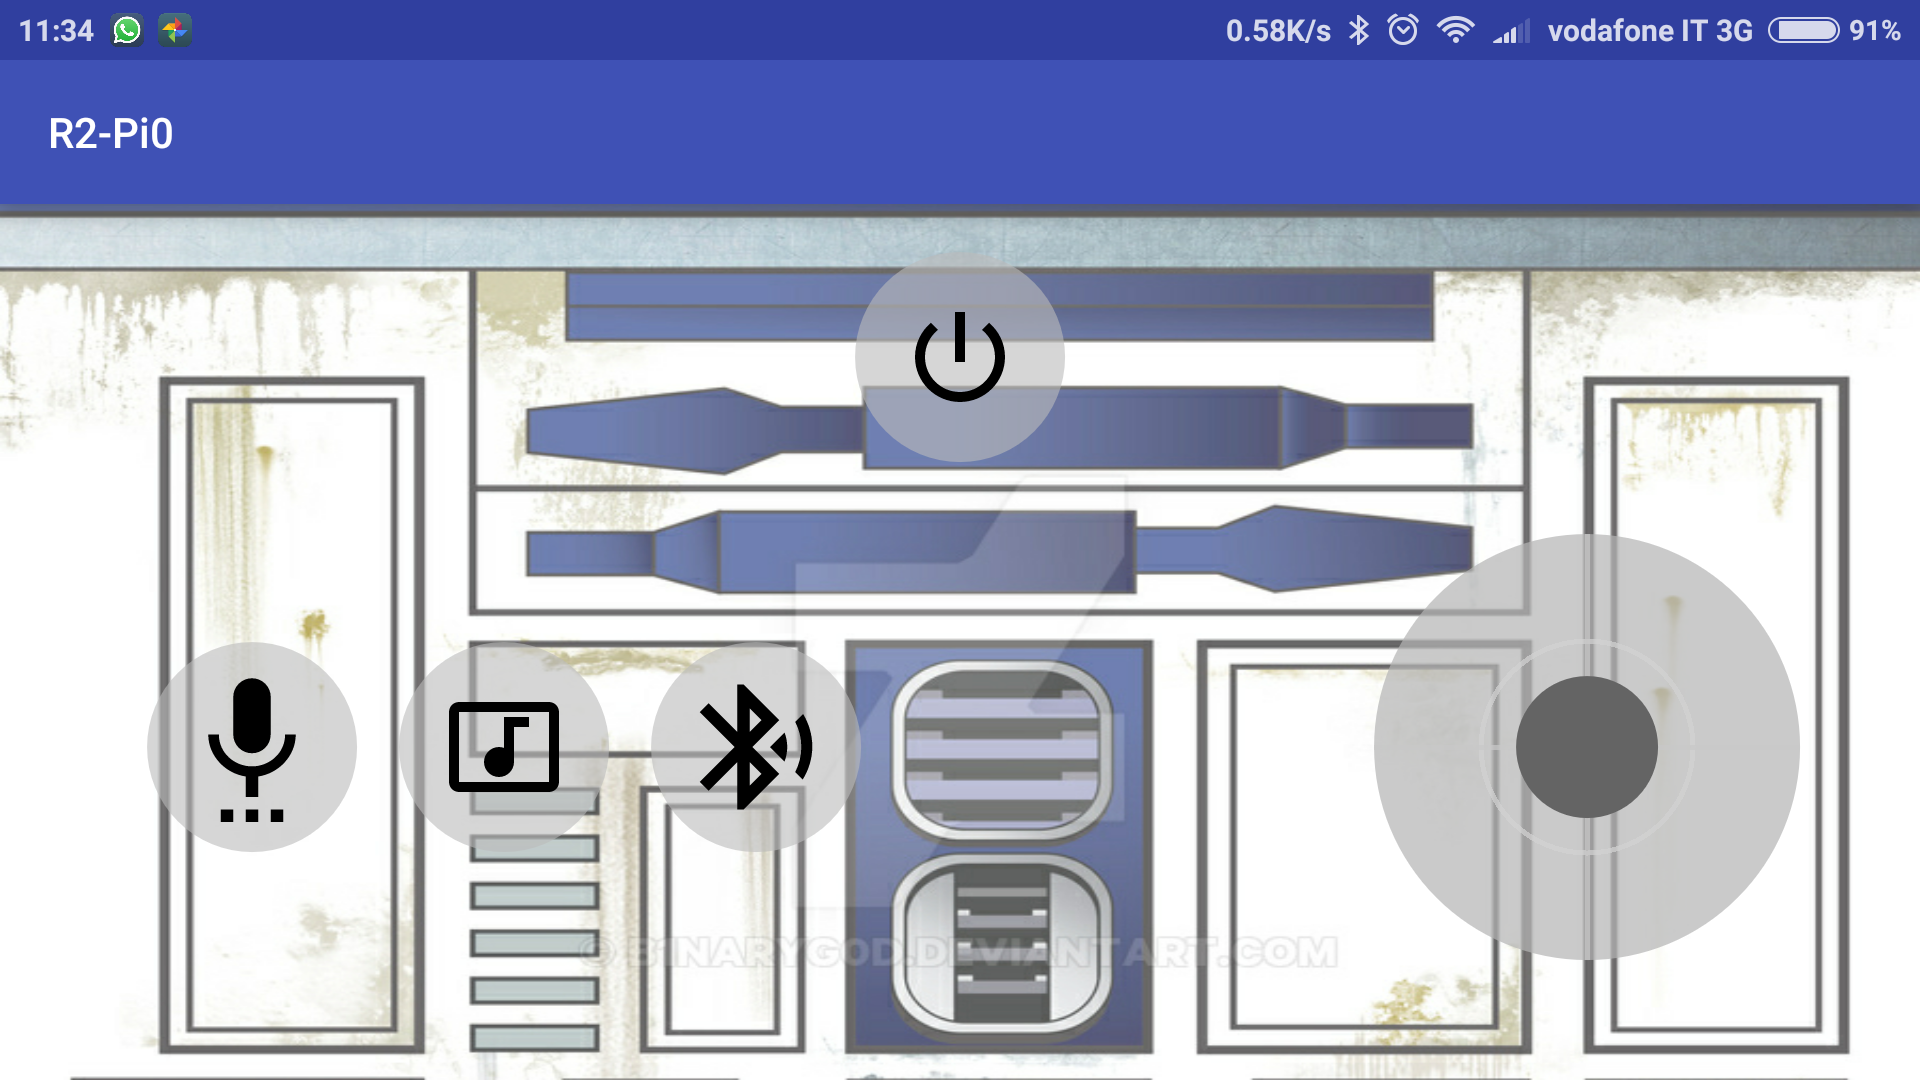
\includegraphics[width=\imgszland]{screenapp}
\centering
\caption{Screen dell'applicazione}
\label{fig:screen}
\end{figure}

\newpage
\subsubsection{Classi}

Le classi che compongono l'applicazione e che permettono tutte le interazioni sono:
\begin{itemize}
\item MainActivity 
\item BluetoothComunication
\item JoyStickView
\item JoyStickTranslator
\item JoyStickTrigonometricTranslator
\item VocalTranslator
\end{itemize}


La classe \emph{MainActivity} rappresenta l'activity principale dell'applicazione, l'unica schermata con la quale interagiremo. 
Il suo compito è quello di instanziare i pulsanti e il joystick, che permettono il movimento e l'utilizzo delle funzioni del robot.
In questa classe creaiamo un oggetto \emph{BluetoothConnection} che ci permettera' l'invio dei vari comandi legati ad ogni pulsante.

La gestione dei comandi vocali avviene direttamente nella MainActivity, fatto che ci permette di non dover creare una nuova activity per la gestione di questa funzione. Viene quindi creata una funzione startSpeechToText che avvia un Intent che inzia a catturare l'audio dal microfono per poi convertirlo tramite i servizi google in testo e salvarlo in una variabile dal metodo onActivityResult, da tale messaggio verra' poi estratto il comando tramite l'oggetto translatore della classe \emph{VocalTranslator} e inviato tramite Bluetooth al robot.

\medskip

La classe \emph{BluetoothComunication} utilizza le classi android per la gestione dei moduli e connessioni bluetooth, in particolare
vengono utilizzate le classi BluetoothAdapter, per creare un oggetto adattatore che ci consentirà di connetterci al robot, BluetoothDevice, che ci servirà per elencare tutti i dispositivi ai quali il nostro smartphone è associato, e BluetoothSocket, che sarà necessario per instaurare la connesione.\\
Affinchè ci possa essere la connesione è necessario effettuare l'associazione tra la parte di programma Python residente su \raspi{} e la parte Java su Android manualmente, da riga di comando, successivamente il \raspi{} verrà visualizzato nell'elenco dei dispositivi associati allo smartphone e basterà selezionarlo nella finestra che compare premendo il pulsante per la connessione Bluetooth.
La classe inoltre prevede la gestione degli errori dovuti all'utilizzo su dispositivi senza Bluetooth e le eventuali perdite della connessione Bluetooth tra smartphone e \raspi{}. Sono poi implementate tutte le funzioni per inviare i comandi al robot.

\bigskip

La classe \emph{VocalTranslator} ha il compito di ricercare, nelle frasi ritornate dal servizio di riconoscimento vocale, le parole chiave che ci permettono di inviare i comandi al robot.
I comandi implementati sono:
\begin{itemize}
\item seguimi
\item rotazione destra e sinistra
\item interruzione della musica
\end{itemize}

Possono essere interpretati sia in lingua italiana che inglese e in diverse forme.

Nel caso dell'inserimento di un comando non riconosciuto il robot emetterà un segnale acustico di errore.

\bigskip

La classe \emph{JoyStickView} permette di disegnare l'elemento JoyStick sulla shermata della nostra applicazione e permettere di ottenere la resistuzione di valori al movimento del cursore.

L'interfaccia \emph{JoyStickTranslator} permette di stabilire i metodi che verranno utilizzati per la restituzione della velocita' e della rotazione.

La classe \emph{JoyStickTrigonometricTranslator} implementa i metodi dell'interfaccia JoyStickTranslator in modo che vengano resituiti dei valori corretti e normalizzati per il successivo invio via Bluetooth al robot.

\section{Struttura}


Nella costruzione dello chassis, per avere una piu' fedele riproduzione dell'originale R2-D2, abbiamo optato per materiali semplici, leggeri e di facile reperibilità, come \emph{cartoncino}, \emph{cartone} e \emph{cartone plastico}.\\
\begin{minipage}{\linewidth}
\medskip
Per rendere la struttura più solida abbiamo poi costruito un'\emph{ossatura} interna con \emph{tubi in PVC} del diametro di 20mm, che unisce le gambe e le spalle, costituendo un'unione fra i motori.
Per le texture abbiamo utilizzato un modello \emph{Pepakura} (reperibile al link: \url{http://www.papercraftsquare.com/star-wars-full-size-r2-d2-free-papercraft-download.html}) in scala 1:1 che abbiamo scalato a 1:1,33 per problemi di stampa delle singole parti.
\medskip
\end{minipage}

Le varie texture sono poi state stampate e incollate con colla vinilica sui differenti materiali.

\bigskip

La struttura esterna delle \emph{gambe} è composta di cartone ondulato monostrato, in quanto costituisce solo una copertura all'ossatura plastica interna e pertanto non richiedeva particolare rigidità strutturale.\\
La semisfera che costituisce la \emph{testa} è costituita da cartone ondulato monostrato, per gli stessi motivi.\\
La parte del \emph{tronco} è stata costruita con cartone plastico, il quale ci ha permesso di ottenere un unico pezzo rigido, tale da conferire una buona stabilità al robot.\\
Il \emph{supporto interno ai componenti} e' costruito in cartone ondulato doppio strato, più resistente e meno flessibile.

Le componenti sono poi incollate fra di loro tramite colla a caldo.
I motori sono agganciati ad un supporto che a sua volta e' collegato alla struttura plastica. 

\bigskip

DA INSERIRE FOTO!

\section{Sviluppi futuri}

Abbiamo pensato ad alcuni interessanti sviluppi futuri:

\begin{itemize}
\item \emph{Aggancio bersaglio ed inseguimento}: l'idea è di dotare il robot di videocamera e, attraverso Open CV o librerie simili, permettergli di agganciare e seguire un oggetto, in particolare pensavamo ad un simbolo da incollare sui nostri vestiti per farci seguire. Ovviamente questo presuppone di passare ad un modello di \raspi{} più performante, come ad esempio il \raspi{} 3, in quanto la computer vision richiede una potenza di calcolo elevata.
\item \emph{Puntamento automatico}: dotare il robot di una pistola ad acqua con cui possa \cbegin fare il dispettoso\cend{} sparando getti d'acqua contro le persone. Ovviamente sempre attraverso Open CV, ma questa volta puntando alle facce.

\end{itemize}



\end{document}
